% !TEX root = SADR.tex
\section{Experiments}
In this section, we first describe the datasets we use to evaluate the proposed approach, followed by the evaluation setup and competing state-of-the-art baselines. We then analyze the performance of our model, followed by ablation studies on different modules and hyper-parameters. Finally, we analyze the importance of each module using the learned weight parameters.

\subsection{Datasets}
We use benchmark datasets available from three online social review platforms: Ciao, Epinions, and CiaoDVD.

Ciao is a product review website where users provide reviews along with ratings for products ranging across a variety of categories. This dataset was crawled by Tang et al.~\cite{Tang} and contains rating information along with the creation timestamp given up to May 2011. Users also establish directed trust relations with other users on the platform and add them to their 'Circle of Trust.'
Epinions is another popular online consumer review website like Ciao~\cite{Tang}. However, this dataset is longer spanning a decade from Aug.\ 1999 to Nov.\ 2013. This dataset also contains trust relations between users\footnote{Both Ciao and Epinions datasets are available at www.cse.msu.edu/~tangjili/trust.html}.
CiaoDVD is a movie review dataset of DVDs crawled from \url{dvd.ciao.co.uk} in December 2013. This dataset contains user reviews of movies accompanied by their overall rating. It also contains directed trust relations between users\footnote{Dataset available from \url{www.librec.net/datasets.html}}.

\begin{table}[tbh]
  \centering
\begin{tabular}{l r r r r } \toprule
  Dataset & \#users & \#items  & \#ratings & \#trusts\\ \hline
 Ciao & 1,653  & 16,862 & 26,190 & 32,955 \\
 Epinions&  22,143  & 296,278 & 464,249 & 83,363 \\
 CiaoDVD & 2,609  & 16,122 & 32,054 & 8,926 \\\bottomrule
\end{tabular}
\vspace{-0.1in}
  \caption{Dataset statistics.}
\label{tab:data}
\end{table}

As we are dealing with implicit feedback (user-item interaction data), we convert all the observed interactions, i.e., ratings, into positive instances. For both datasets, we only keep users with at least five rated items. The final data statistics are summarized in Table~\ref{tab:data}. Epinions is by far the largest dataset.

%-------------------------------------------------------------------------
\subsection{Evaluation Protocol}
We split each user sequence into training, validation, and test set. For each user, the most recent item is held out for testing. The second most recent item is held out for validation while we train the model on the remainder of the sequence. The validation set is used for tuning the model hyper-parameters, e.g., learning rate, embedding dimension, sample size of user's friends, etc. % of the model.

We evaluate model performance on the test set via two widely used evaluation metrics:  HitRate@10 (HR@10) and Area under Curve (AUC). HitRate@10 is computed as follows:
\begin{align}
  HR@10 = \frac{1}{\vert {\mathcal U} \vert} \sum_{u \in {\mathcal U}} \mathbbm{1}  (L_{u,i_u^{t}} < 10),
\end{align}
where $i_u^{t}$ is the ground truth item that user $u$ clicked at test time $t$, $L_{u,i_u^{t}}$ is the rank of the ground truth item in the predicted ranked list, and  $\mathbbm{1}(.)$ is the indicator function. The HR@10 metric checks if the ground truth item is present in the top-10 ranking.
In contrast, AUC measures the rank of the test item in the predicted ranked list. This is a harder metric as it takes into account  the exact position of the ground truth item. Formally,
\begin{align}
AUC = \frac{1}{\vert {\mathcal U} \vert} \sum_{u \in {\mathcal U}} \frac{1}{\vert {\mathcal I} \vert} \sum_{j \in {\mathcal I}} \mathbbm{1} (L_{u, i_u^{t}} > L_{u,j}).
\end{align}
where $L_{u,j}$ is the rank of item $j$ in the predicted ranked list for user $u$.
Due to the sparsity of user-item interaction data (number of items is huge) and computational feasibility, following~\cite{He:2016}, HitRate@10 is reported on a sample subset of negative items instead of the whole set. For each user-item pair in the test set, we sample 99 negative items that the user has not rated before.  Similarly, for AUC computation, we sample a set of 5,000 unobserved items for each user for both our model and the baselines.

\subsection{Baselines}
We compare to a large variety of state-of-the-art collaborative filtering (CF), temporal, social, and socio-temporal recommenders:
\begin{itemize}
\item BPR-MF~\cite{Rendle} is a classic matrix factorization model which uses a pairwise ranking loss.
\item NeuMF~\cite{NeuMF} is a recently proposed CF based model with neural architecture. It merges matrix factorization and multi-layer perceptron modules to predict item ranking.
\item NAIS~\cite{NAIS} is an item-to-item CF based model which employs user-specific attention between items to identify similar items\footnote{\url{github.com/AaronHeee/Neural-Attentive-Item-Similarity-Model}}.
\item TBPR~\cite{TBPR} extends the BPR model to capture strong and weak ties separately in a user's social network in order to distinguish the degree of influence of a user's connections on her behavior.
\item SERec~\cite{SERec} is a state-of-the-art CF based social recommender model that augments collaborative filtering with social exposure through regularization and boosting.
\item DiffNet~\cite{Diffnet} is a state-of-the-art graph convolution based social recommender that propagates user influence through their social network. Due to the absence of attributes in our dataset, we replace the user and item feature vectors with one-hot embeddings in their model\footnote{\url{github.com/PeiJieSun/diffnet}}.

\item GraphRec~\cite{fan2019} is another recently proposed social recommender that uses graph convolution networks to incorporate information from both a user-item and a user's social graph.
The original model was proposed for rating prediction, and we adopt it for our item ranking task. For that purpose, we change the loss function to a log loss and augment the training data with randomly sampled negative items following other ranking prediction models \cite{NeuMF}.

\item SASRec~\cite{SAS:2018} is a state-of-the-art model for the temporal recommendation that uses a self attentive module to capture long-term interests of a user\footnote{\url{github.com/kang205/SASRec}}.

\item SR-GNN~\cite{SRGNN} is a graph neural network based temporal recommender that aggregates information from all previous timesteps of the user\footnote{\url{github.com/CRIPAC-DIG/SR-GNN}}.

\item SPMC~\cite{Cai:2017} is an extension of a Markov chain based~\cite{Rendle2} model which captures both temporal and social dynamics for recommendation\footnote{\url{github.com/cwcai633/SPMC}}.


\item ARSE~\cite{Sun:2018} is a state-of-the-art social session recommendation model. It employs a session LSTM module to model change in user preferences across sessions while incorporating social influence as an input to the LSTM module\footnote{\url{github.com/DeepGraphLearning/RecommenderSystems/}}. Similar to their paper, we divide the dataset into monthly intervals and predicted for the next session\footnote{We also experimented with constraining each session to comprise of just a single item, but that resulted in slightly worse performance.}.
\item DGRec~\cite{Song:2019}: Another social session recommender method that uses graph attention networks to merge preferences of social neighbors from the previous session with a user's preference in the current session. We use similar month-wise intervals to denote each session\footnote{We also evaluated other intervals, but they all performed similarly.}.
\end{itemize}

BPR-MF, NeuMF and NAIS are Collaborative Filtering models, while TBPR and SERec are social recommenders.
Diffnet and GraphRec are graph convolution based social recommenders. SASRec and SR-GNN are temporal recommender models. We omit a comparison with Fossil and GRU~\cite{GRU4Rec} as they are RNN based temporal recommendation methods. The results for our user-temporal module are equivalent to their models.
SPMC is most similar to our model as it also models temporal behavior and socio-temporal influence. However, it is a shallow model as it extends a Markov chain to model linear dependence. ARSE and DGRec are also socio-temporal recommenders proposed for session recommendations.

We use the Adam optimizer for our models with a batch size of 256 for Ciao, CiaoDVD, and 1024 for Epinions. We used the implementation provided by the RecQ python library\footnote{\url{github.com/Coder-Yu/RecQ}} for BPR-MF, NeuMF, TBPR, and SERec models. We used the authors' implementation for all the other models. Specifically, for ARSE and GraphRec, we wish to thank the authors as they generously shared their implementation.
We keep the embedding dimension $D=32$, for all the baselines to be comparable with our model. We report the best result of the baselines using either hyper-parameters based on the authors' specifications or values, which performed better on our validation set.

\subsection{Performance Analysis}

Table~\ref{tab:baseline} details a comparison of HR@10 and AUC for our model and the state-of-the-art baselines on all three datasets. We report mean results over five runs.
Our model significantly outperforms all the baselines on the AUC metric by at least around 2\% for CiaoDVD, 14\% for Epinions, and 18\% for Ciao.
On the Ciao and Epinions dataset, our \ours {} model also improves the HR@10 metric by at least 4\%. Note that each of the baselines models one or a subset of three factors (temporal, socio-temporal, and item similarity), while our \ours {} model considers all factors jointly. Each of our modules outperforms their respective baselines. Further, the combined \ours {} model considerably outperforms the individual components. This improvement indicates that our model is effective at combining the individual modules, each capturing a distinct factor affecting a user's preference.

\begin{table*}[tbh]
  \centering
  \setlength{\tabcolsep}{5pt}
\begin{tabular}{p{34mm} l c c c c c c} \toprule
\multirow{2}{*}{Model Type}  & \multirow{2}{*}{Models} & \multicolumn{2}{c}{Ciao} & \multicolumn{2}{c}{Epinions}  & \multicolumn{2}{c}{CiaoDVD}\\
    &    &  HR@10   &    AUC         &    HR@10   & AUC &    HR@10   & AUC \\ \hline
  \multirow{3}{*}{Classical} & BPR-MF~\cite{Rendle} & 0.297 & 0.630 & 0.509 & 0.731 & 0.517 & 0.759 \\
   & NeuMF~\cite{NeuMF}  & 0.342 & 0.570 & 0.470 & 0.709 & \textbf{0.551} & 0.760 \\
   & NAIS~\cite{NAIS}  & 0.241 & 0.626 & 0.510 & 0.723 & 0.487 & 0.742 \\ \hline
  \multirow{4}{*}{Social} & SERec~\cite{SERec} & 0.295 & 0.550 & 0.421 & 0.613 & 0.385 & 0.647 \\
  & TBPR~\cite{TBPR}  & 0.322 & 0.601 & 0.47 & 0.717 & 0.518 & 0.745 \\
  & DiffNet ~\cite{Diffnet}  & 0.342 & 0.583 & - & - & 0.527 & 0.759 \\
  & GraphRec~\cite{fan2019}  & 0.234 & 0.534 & 0.452 & 0.702 & 0.33 & 0.708 \\
  \hline
\multirow{2}{*}{Temporal} & SASRec~\cite{SAS:2018} & 0.324 & 0.575 & 0.508 & 0.724 & 0.546 & 0.761 \\
  & SR-GNN~\cite{SRGNN} & 0.320 & 0.590 & 0.509 & 0.732 & 0.546 & 0.759 \\ \hline
\multirow{3}{*}{Social + Temporal}  & SPMC~\cite{Cai:2017} & 0.223 & 0.599 & 0.483 & 0.717 & 0.53 & 0.758 \\
& ARSE~\cite{Sun:2018} & 0.328 & 0.583 & 0.522 & 0.726 & 0.527 & 0.754 \\
& DGRec~\cite{Song:2019} & 0.329 & 0.610 & 0.479 & 0.726 & 0.521 & 0.753 \\ \hline
  \multirow{3}{*}{Our Indiv. Modules}  & User-Temporal & 0.308 & 0.666 & \textbf{0.559} & 0.726 & 0.535 & 0.751 \\
    & User-Social & 0.344 & 0.637 & 0.503 & 0.736 & 0.551 & 0.741 \\
  &Item-Similarity & 0.208 & 0.604 & 0.430 & 0.758 & 0.474 & 0.767 \\ \hline
Ours Combined  & \ours & \textbf{0.355} & \textbf{0.745} & 0.549 & \textbf{0.834} & 0.538 & \textbf{0.774} \\
 \bottomrule
\end{tabular}
  \caption{Comparison of results of our model to state-of-the-art baselines and variants of our own model on three datasets. Higher values are better for both metrics. Our model significantly outperforms the baselines that model a subset of three factors. `$-$' indicates an out of memory error.
  }
\label{tab:baseline}
\end{table*}

Amongst our proposed modules, in general, the user-social module performs best on the HR@10 metric, while the item-similarity module outperforms the other modules on the AUC metric. This difference could be because the user-social module improves the ranking of items currently popular among a user's social connections.
In contrast, the item-similarity module emphasizes items that frequently co-occur in the entire dataset, irrespective of the user preferences. This increases the bias of the item ranking only slightly, as co-occurrence is a weak signal for a specific user (it is averaged across all users).
This difference further underlines that it is essential to model a variety of factors for an effective recommendation.

\textbf{Collaborative:} CF-based approach BPR-MF performs the best among the baselines when considering the AUC metric while NeuMF performs competitively for HR@10.
This superior performance highlights that classical matrix factorization approaches are still very competitive for the recommendation. The user-specific attention-based NAIS model did not outperform the non-attention based CF models.

\textbf{Social:} Our proposed user-social module outperforms all baseline social recommenders for both metrics.
Among the baselines, the TBPR model that models the user's social graph with different weights for strong and weak ties performs better than the SERec that considers each friend's contribution equally. This reaffirms our assumption that each friend exerts a different influence on the user. In general, we found the recently proposed SERec to underperform on the three datasets used here. It proposes that social connections have a limited influence on a user's preference.  Social influence is weakly modeled through an exposure prior on the items. However, we think the low performance indicates the contrary, i.e., social influence plays a significant part in shaping a user's preference.

Our GCN based user-social module is inherently different from the other GCN based baselines, DGRec, and GraphRec. Our user-social module is time-dependent with dynamic user features while both baselines operate on static features (entire item history). Further, our architecture differs: we employ attention between a user and her social connections, whereas DiffNet does not use attention, and GraphRec computes attention based on user history rather than the user itself. Our superior performance supports the difference.

However, the DiffNet model performs the best among social recommenders. However, it is unable to scale to our largest dataset, Epinions. Note that we used the authors' implementation, and our largest dataset is bigger than the one reported in their paper. In contrast, the other GCN based model GraphRec performs poorly on all the datasets. Note that for results obtained in their paper, they only consider users with non-zero social connections and items previously seen in the training data, while we do not make any such assumptions.

\textbf{Temporal:} Our user-temporal module uses information from only the previous timestep for prediction at the current timestep while the baseline temporal recommenders aggregate information from all previous timesteps. However, we argue that information from a distant past is not useful. Comparable performance of our user-temporal module with the temporal baselines confirms our argument.
In general, both the temporal recommenders, SASRec and SR-GNN, perform better than social recommenders and are comparable to the best performing BPR baseline on the Epinions and CiaoDVD dataset when using the AUC metric. While they perform competitively with other baselines on HR@10.

\textbf{Social + Temporal:} SPMC, which combines temporal and social influence, performs worse than baselines, which model either of the two factors. This worse performance is expected as it is a shallow model with linear dependence. The other socio-temporal models ARSE and DGRec perform similarly, with ARSE performing slightly better for the HR@10 metric. Note that despite modeling socio-temporal influence, these methods do not outperform even other social and temporal only baselines. This could be since these models were originally proposed for the session-based recommendation. Sessions are typically defined as a sequence of activities performed by a user in a single visit to the website or platform.

Thus, for the session prediction settings, models work on recommending the next item to consume by the user in the same session. They typically assume either none or limited past session information of the users and assume static user preferences per session.
In contrast, we model the evolution per item for each user and expect a significant change in a user's preference over time.

Further, DGRec only models socio-temporal influence (based on a friend's last session) and ignores the evolution of a user's preference across sessions. In contrast, ARSE models a user's evolution across sessions but aggregates information per session resulting in limited flexibility. Also, it is worthy to note that none of these models exploit similarity in the item space that is used in our proposed model.
Thus, the worse performance of these session-based socio-temporal methods indicates that they are not well suited for temporal recommendation owing to information aggregation within sessions.

\subsection{Module Analysis}
\label{sec:mod}

\begin{figure}[tbh]
 \centering
   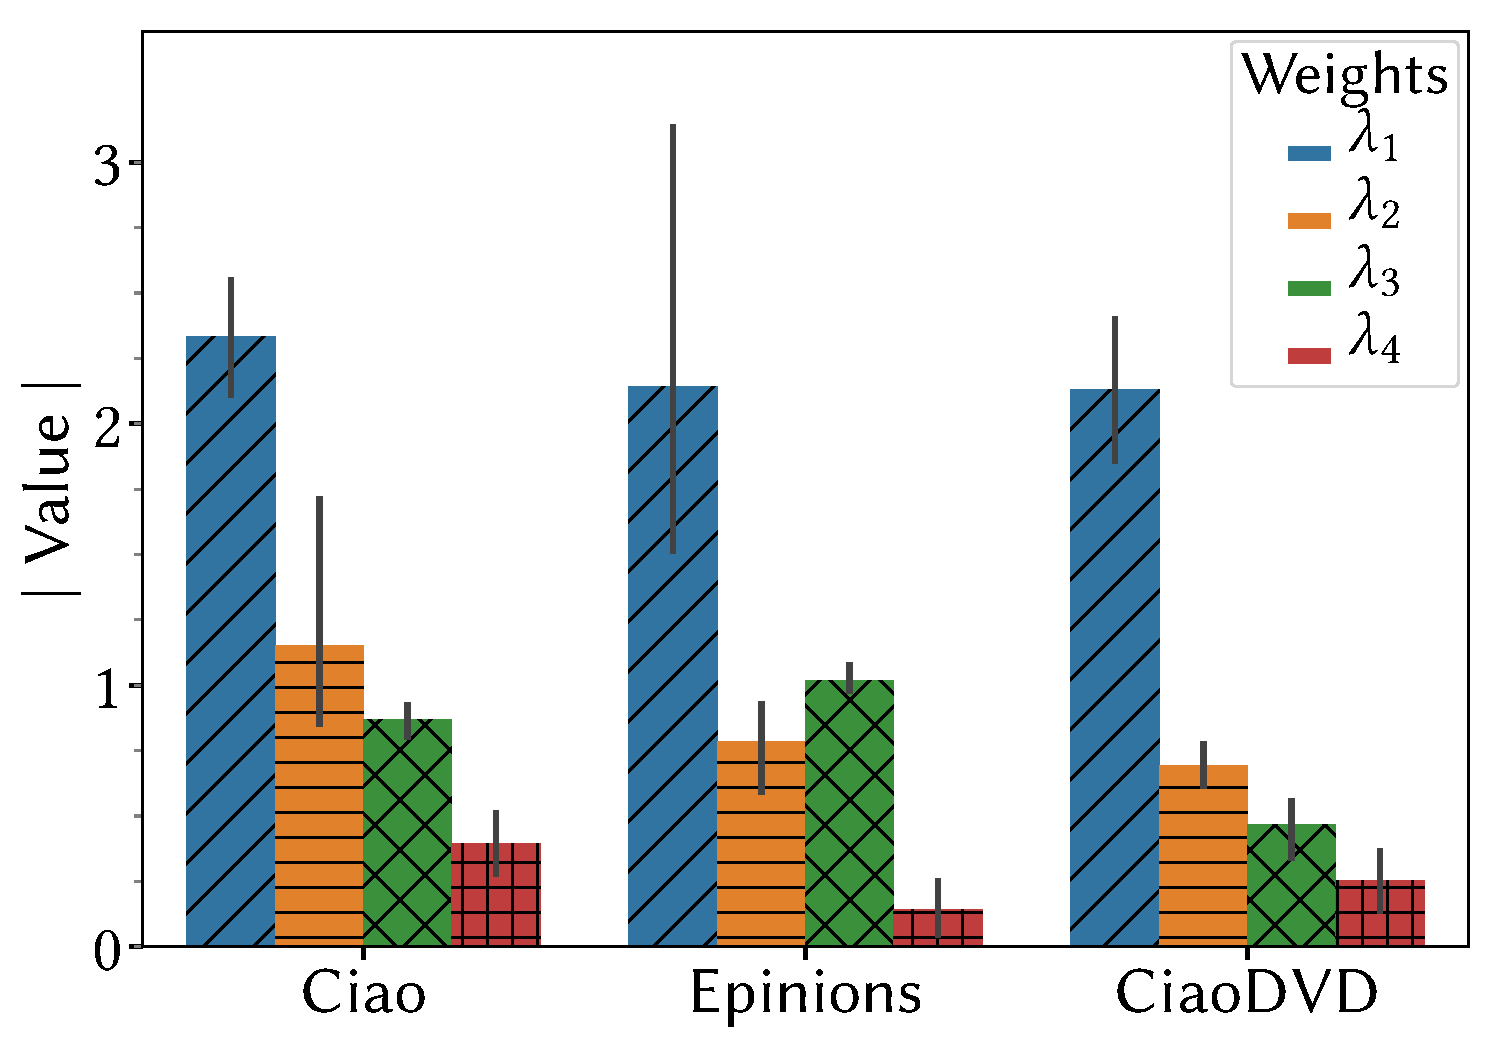
\includegraphics[scale=0.36]{figures/weight.pdf}
 \caption{Learned value of the weights $\lambda_k$ for $k \in \{ 1, \ldots ,4 \}$ for different scores in our model. Weight $\lambda_1$ corresponding to user-temporal embedding contributes most to the final score.}
 \label{fig:weight}
\end{figure}

We now evaluate the importance of each module (user-temporal, user-social, and item-similarity) in our combined model using learned weights, $\lambda_k$. \Cref{fig:weight} shows the learned magnitude of the weights $\lambda_k$ for $k \in \{ 1, \ldots ,4 \}$ for each of the $S_k$ (\Cref{eq:fuse}) scores for all the datasets. Weight $\lambda_1$ corresponds to a user-temporal embedding ($h_u^t$) %\as{`user temporal' or `temporal user'?}
and contributes most to the final score. This high magnitude is expected as a user's history of interactions play a crucial role in modeling user preferences accurately.
$\lambda_2$ corresponds to the context-specific user-temporal embedding ($h_{u,i}^t$) and is the second most important factor for Ciao and CiaoDVD datasets. In contrast, $\lambda_3$, which corresponds to a  user-social embedding ($s_{u}^t$) is the second highest factor for Epinions. This difference indicates that social influence plays an important factor for users in the Epinions dataset while it is slightly less important for the Ciao and the CiaoDVD datasets. $\lambda_4$, which  corresponds to the context-specific user-social embedding ($s_{u,i}^t$) contributes the least across all datasets. Note that all scores use item-similarity embeddings.

Next, we perform ablation experiments by removing each individual module at a time from the final model, as shown in \Cref{tab:individual}.
All variants perform worse than the final \ours {} model, emphasizing the need for each of the modules.
For all the datasets, removing the user-temporal module results in the largest drop in performance. This is expected as a user's history encapsulates a great deal of information for the recommendation. Thus, personalized recommendations fare better than generic ones.

\begin{table}[tbh]
  \centering
\begin{tabular}{l  c c c c c c} \toprule
\multirow{2}{*}{Model Variants} & \multicolumn{2}{c}{Ciao} & \multicolumn{2}{c}{Epinions} & \multicolumn{2}{c}{CiaoDVD} \\
&  HR@10   &    AUC         &    HR@10   & AUC &    HR@10   & AUC \\ \hline
\{social + item\} & 0.329 & 0.574 & 0.478  & 0.713 & 0.526 & 0.738\\
\{temporal + item\} & 0.335 & 0.631 & 0.557 & 0.798  & 0.531 & 0.743\\
\{temporal + social\} & 0.327 & 0.679 & 0.536 & 0.736  & 0.540 & 0.745\\
\ours & 0.355 & 0.745 & 0.549 & 0.834  & 0.538 & 0.774 \\
 \bottomrule
\end{tabular}
    \caption{Performance of our \ours {} model for all three datasets, when removing one module at a time. All of these variants perform worse  than the combined model.}
    \label{tab:individual}
\end{table}

Apart from the user-temporal module, for CiaoDVD, the model without the item-similarity module performs best, while for Epinions and Ciao, the model without user-social module performs the best. Thus, for the movie reviewing platform CiaoDVD, preferences of a user's social connections play a significant role in predicting her movie preferences.

In contrast, for Epinions and Ciao, both of which contain broad categories of products, items frequently bought together by users are better predictors of purchasing behavior. This seems intuitive as movie preferences are subjective in general, while users tend to believe strangers on online reviewing platforms for products like electronics, furniture, etc.


\begin{figure}[tbh]
  \centering
    \begin{tabular}{c c c c}
      item-similarity & user-social & user-temporal \\
    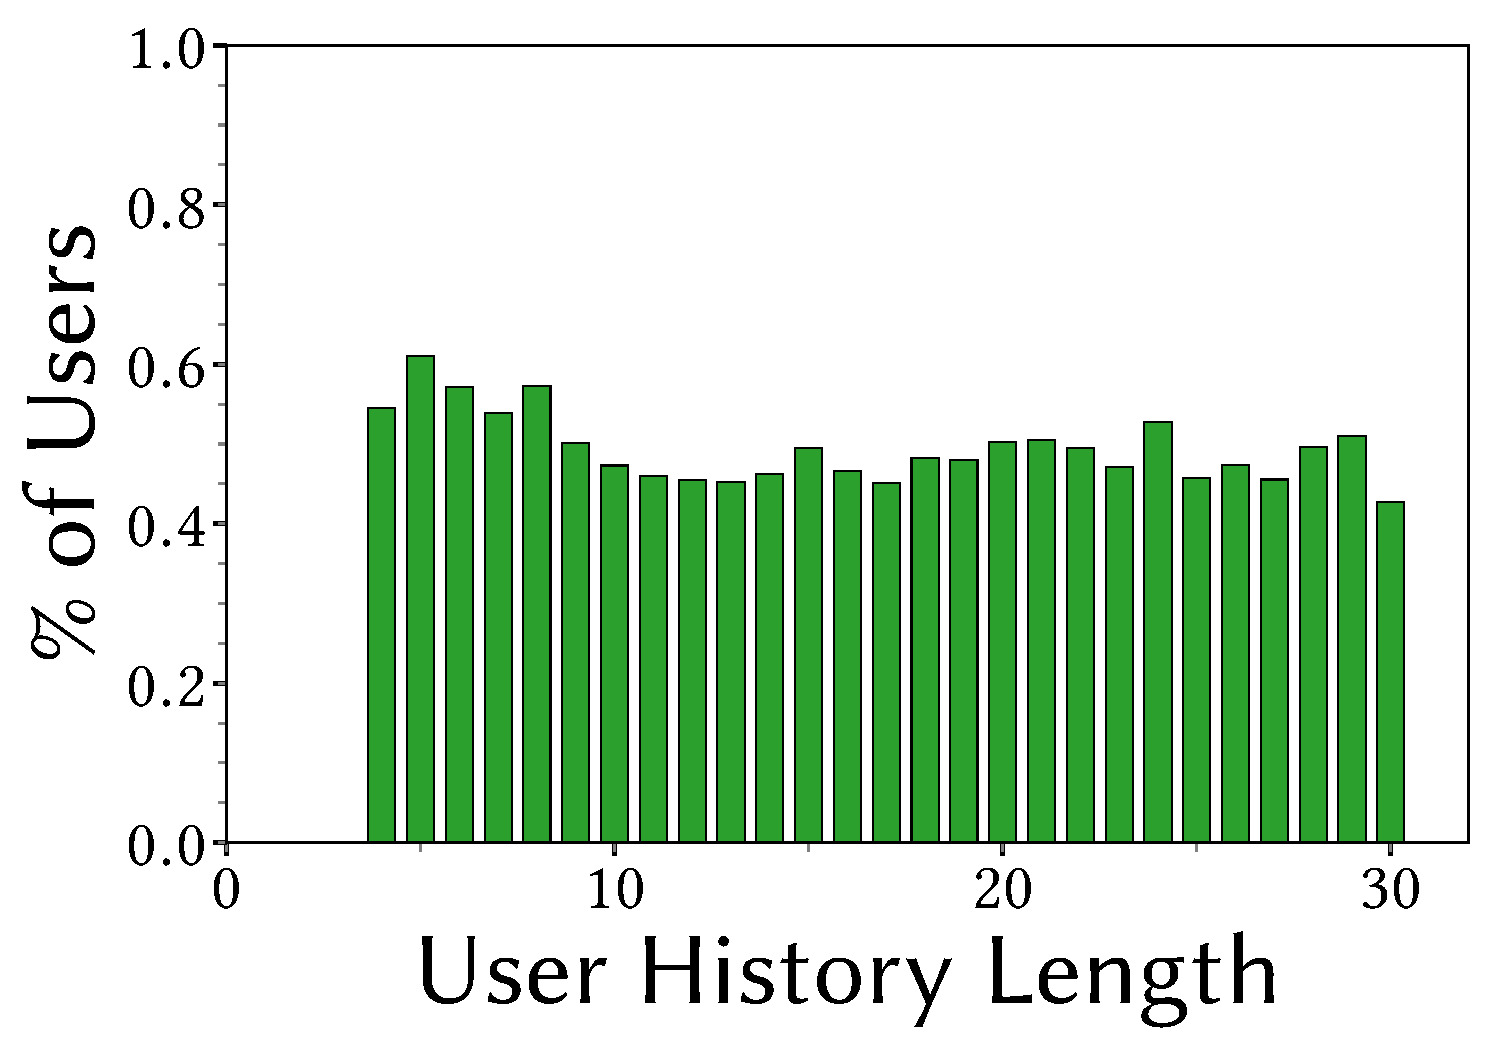
\includegraphics[height=4cm,width=0.3\linewidth]{figures/epinions_itemSocial_Total_users_length.pdf}
 &
    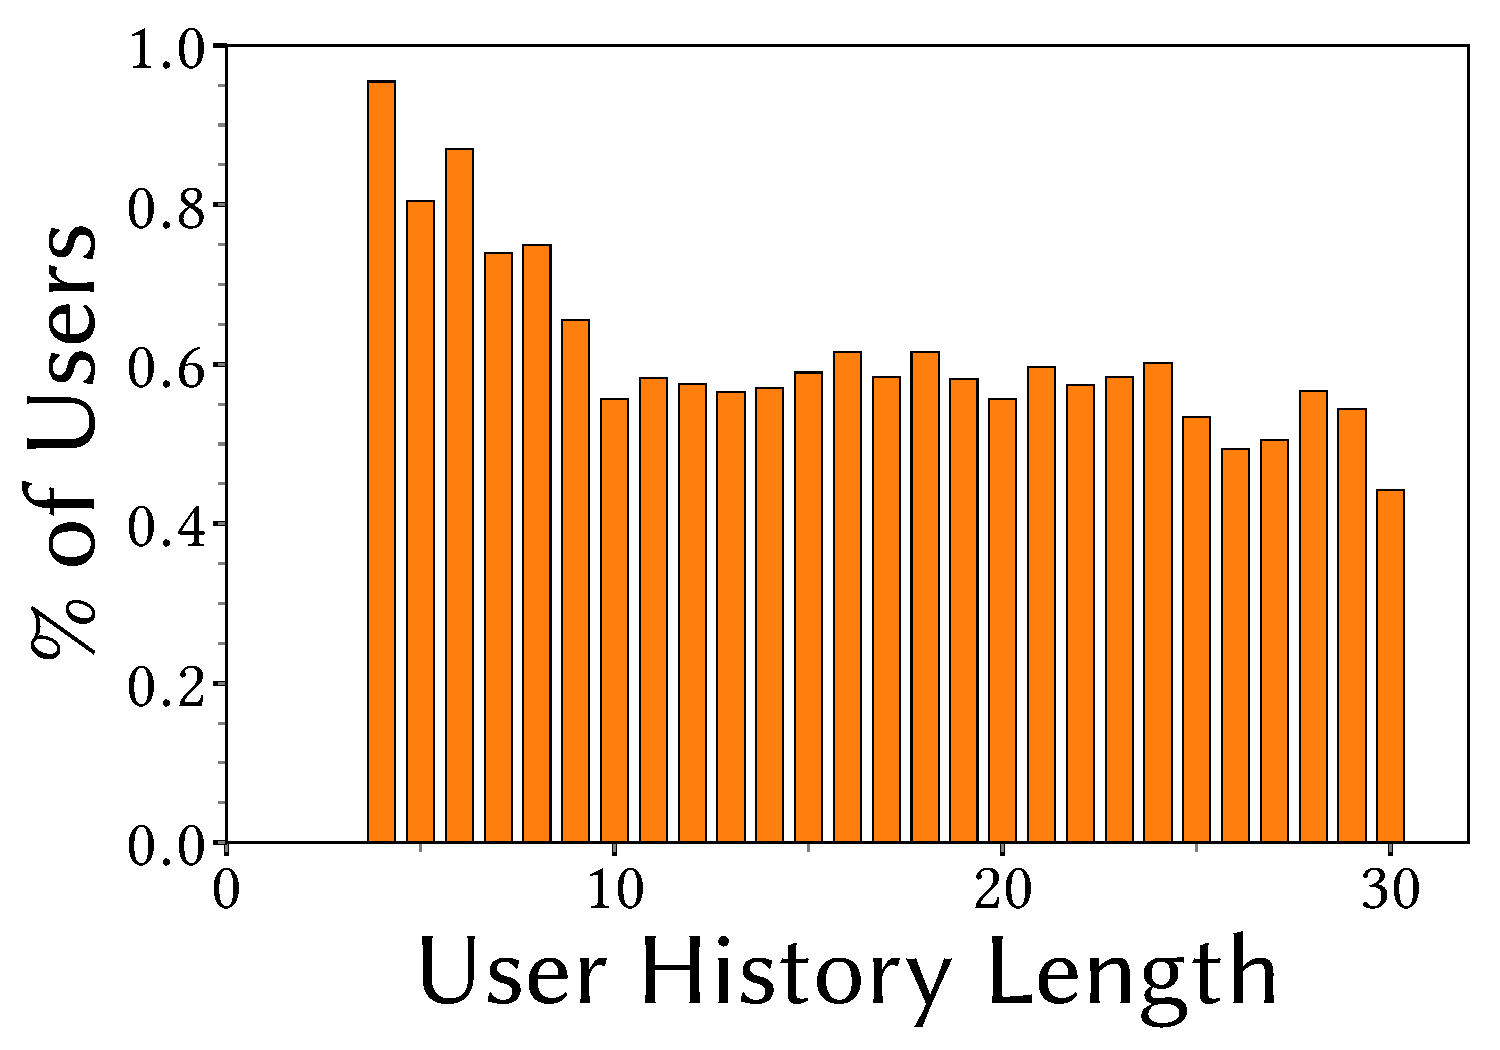
\includegraphics[height=4cm,width=0.3\linewidth]{figures/epinions_userSocial_Total_users_length.pdf}
  &
    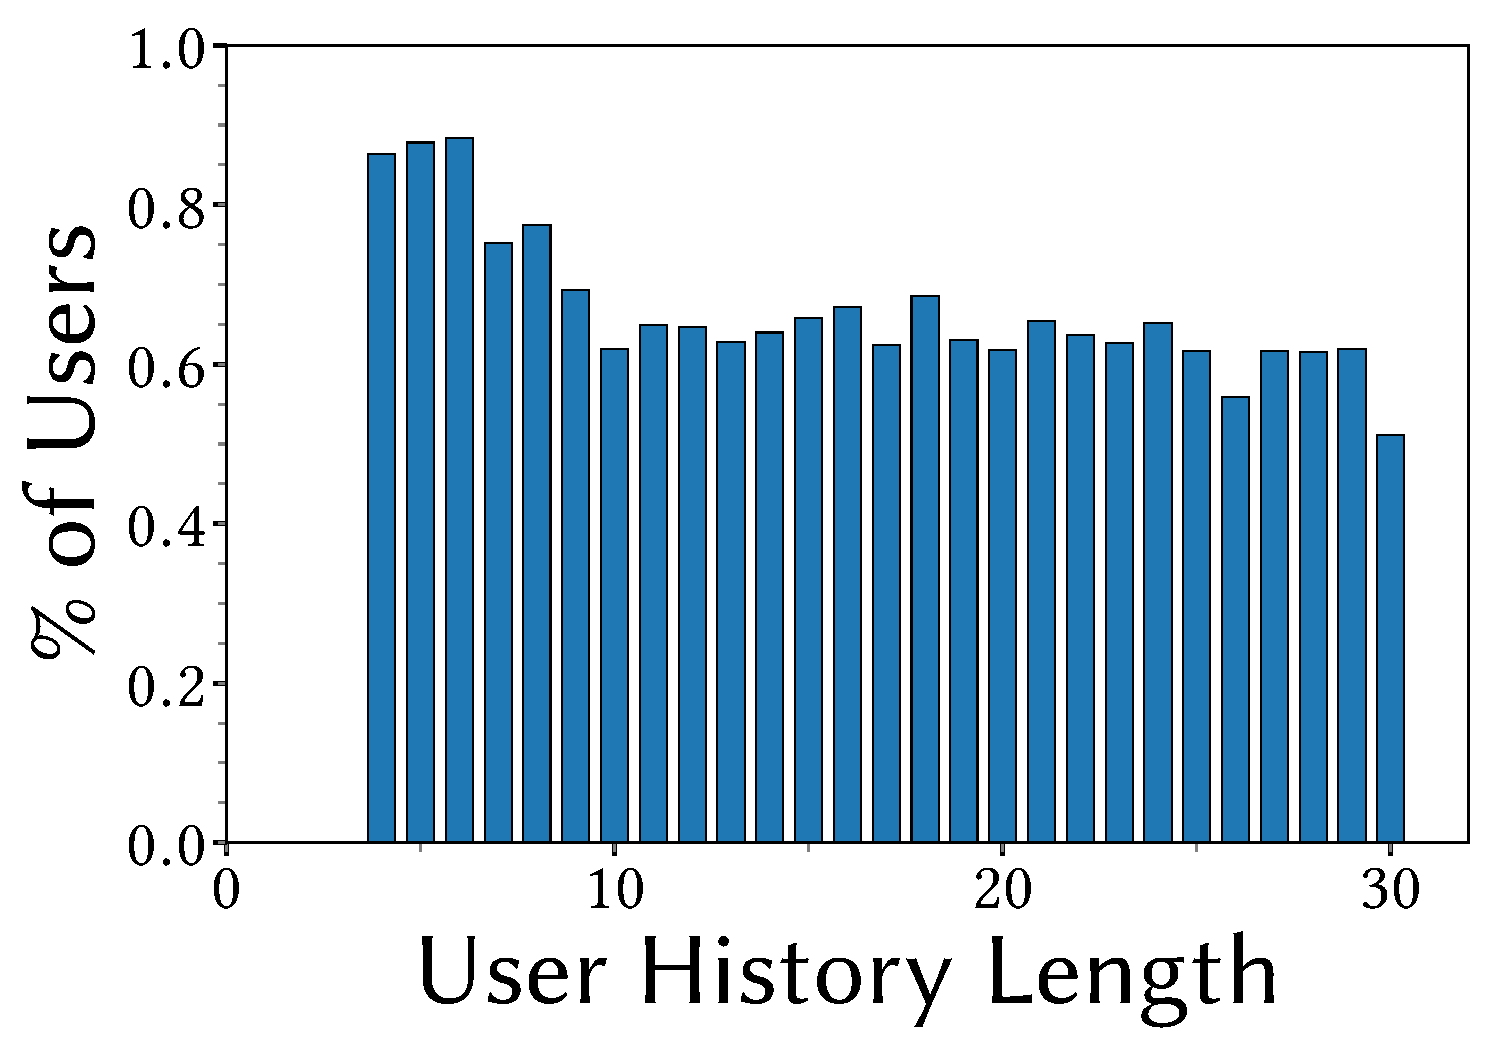
\includegraphics[height=4cm,width=0.3\linewidth]{figures/epinions_temporal_Total_users_length.pdf}\\
    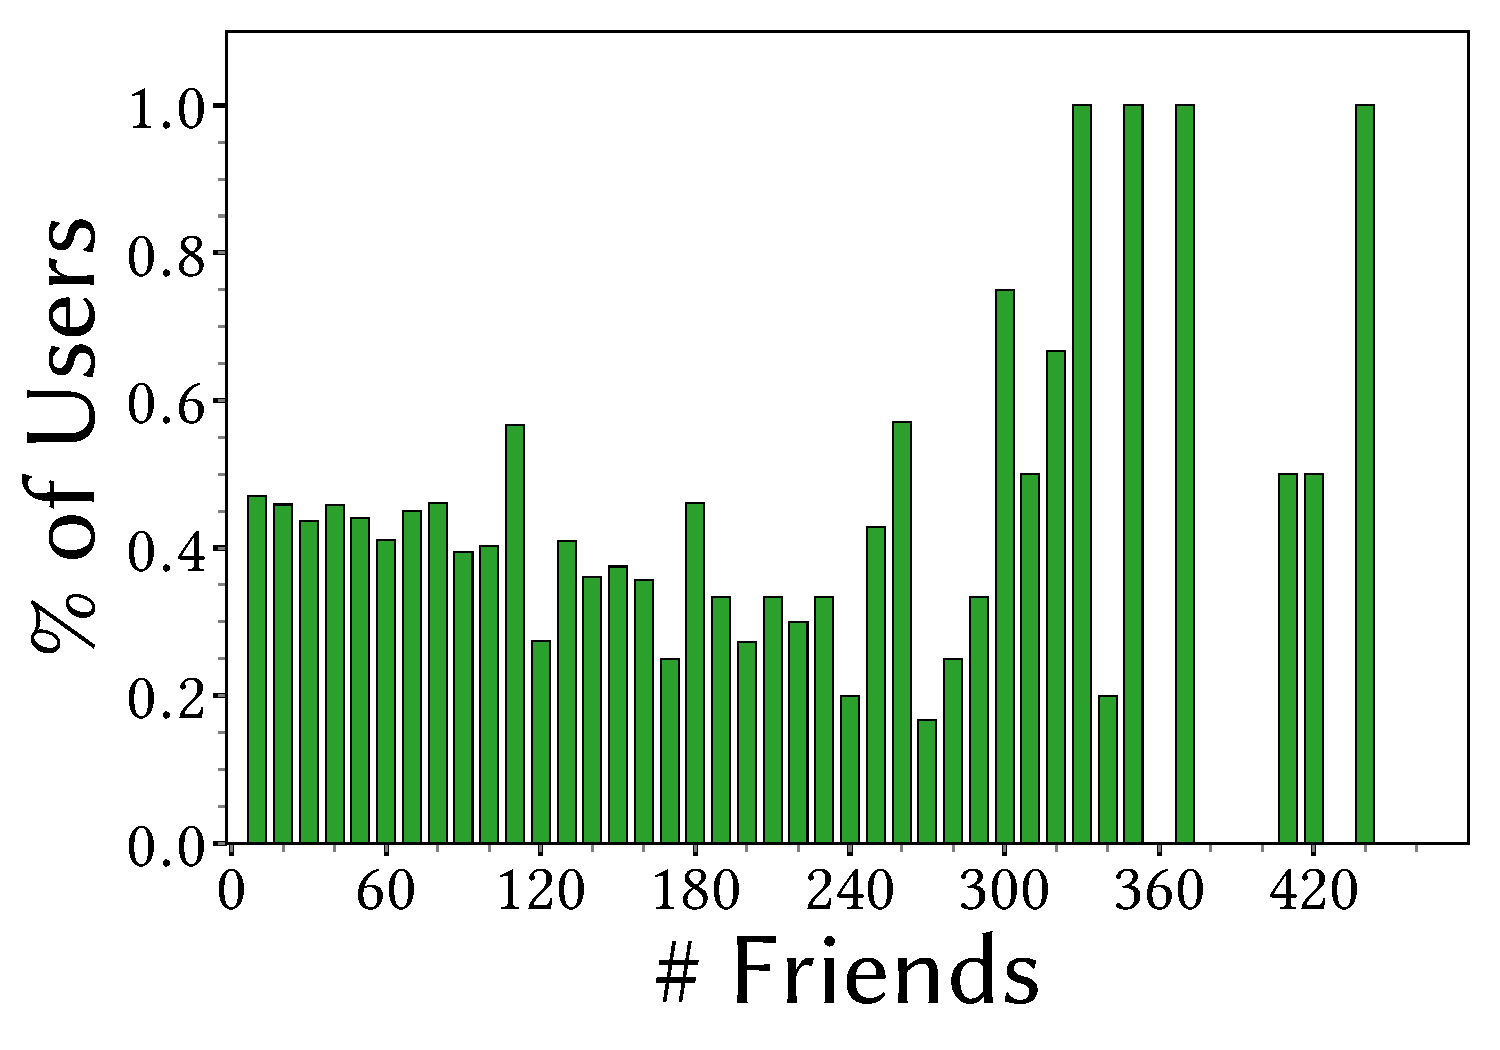
\includegraphics[height=4cm,width=0.3\linewidth]{figures/epinions_itemSocial_Total_users_friend.pdf}
 &
    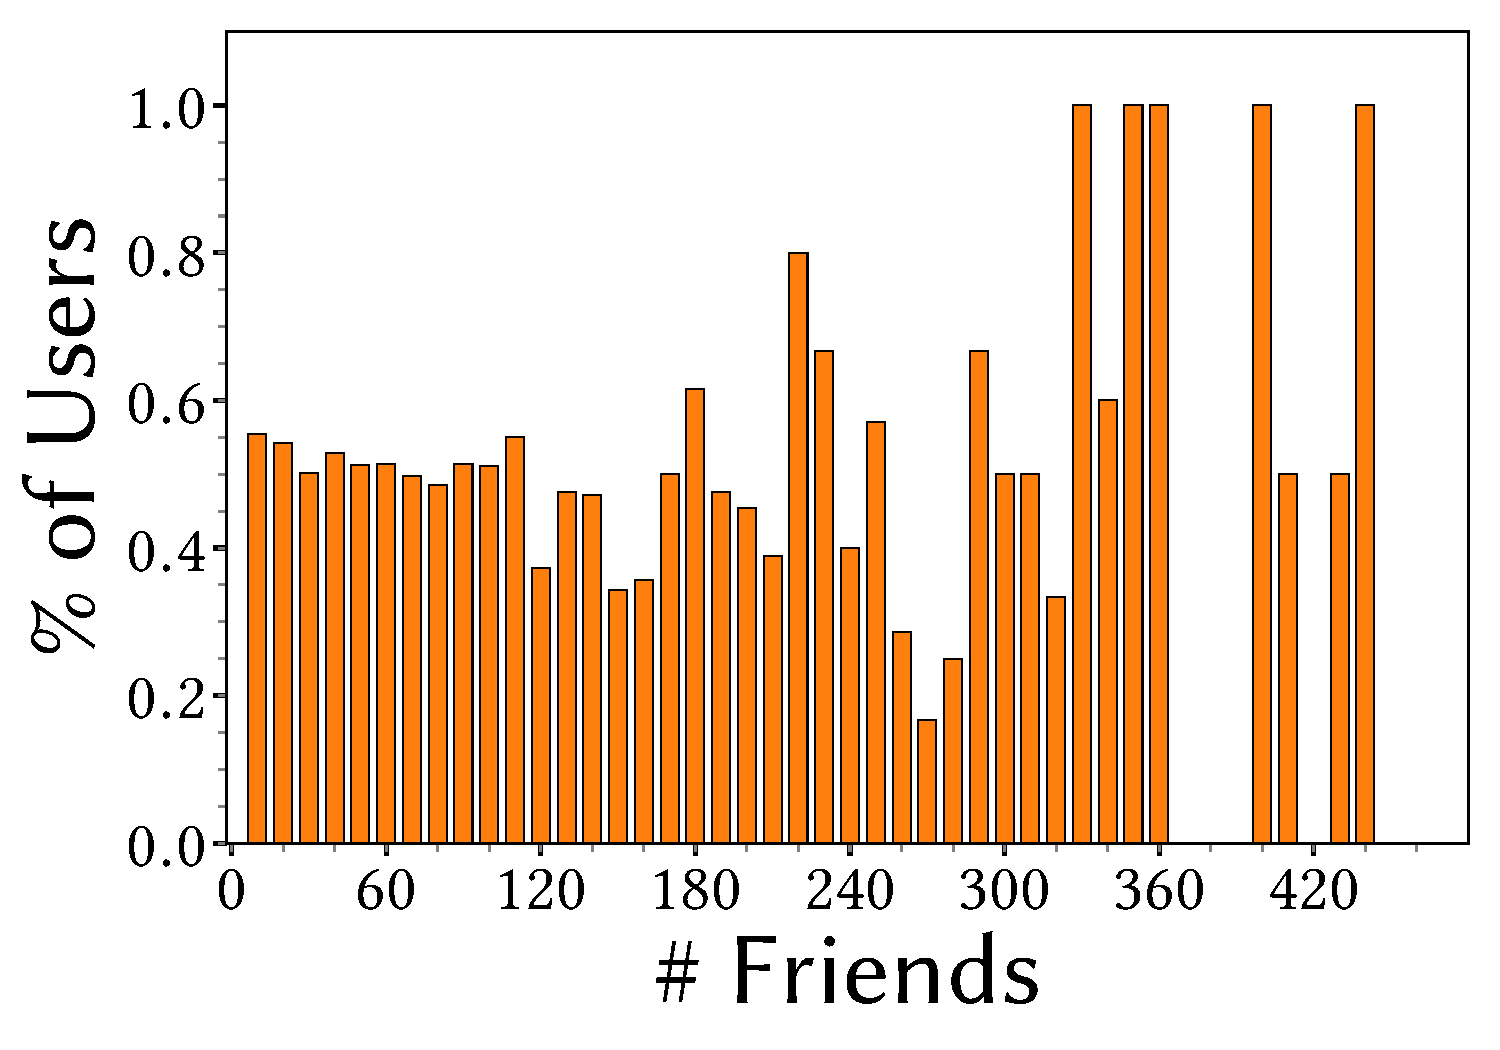
\includegraphics[height=4cm,width=0.3\linewidth]{figures/epinions_userSocial_Total_users_friend.pdf}
  &
    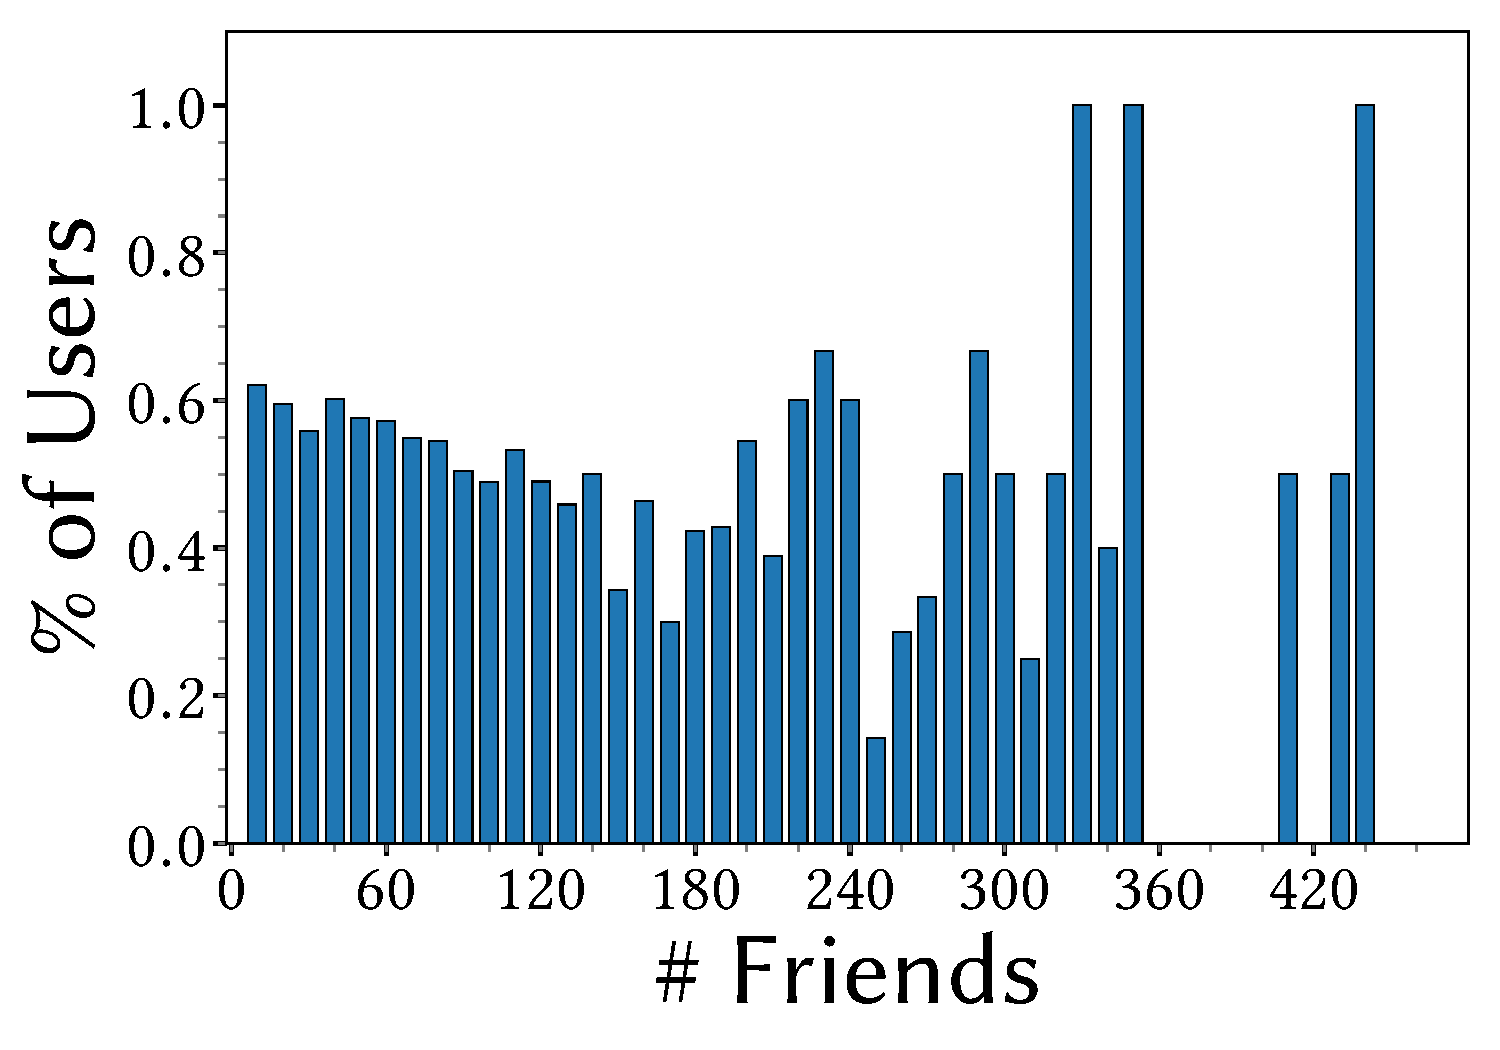
\includegraphics[height=4cm,width=0.3\linewidth]{figures/epinions_temporal_Total_users_friend.pdf}\\
    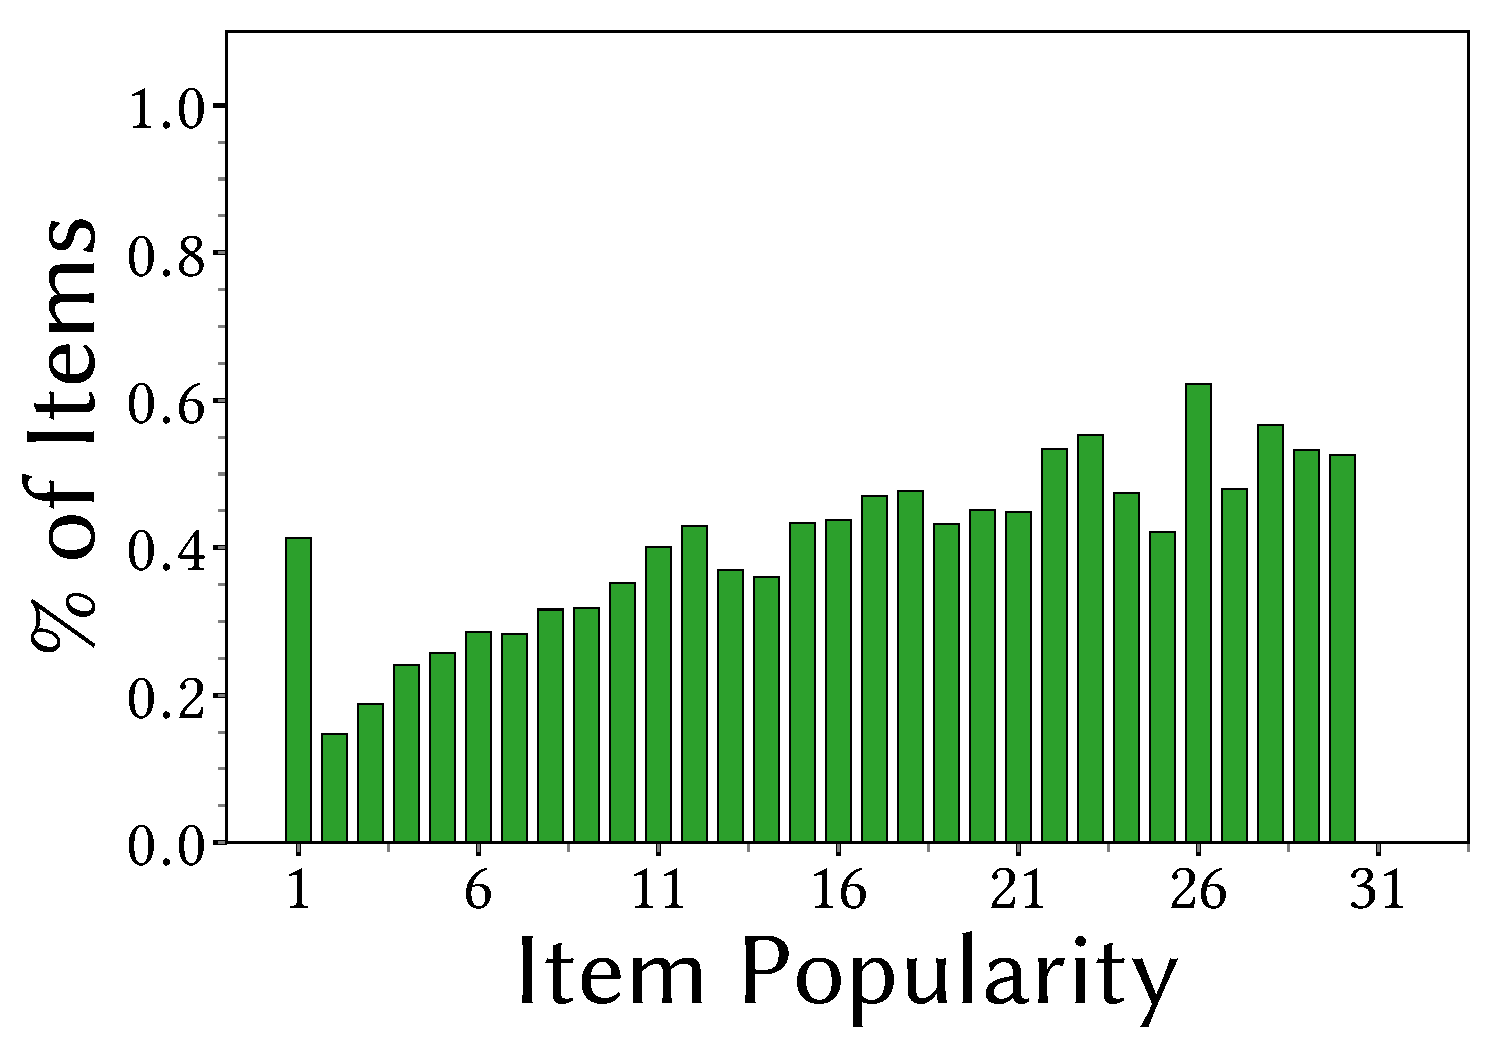
\includegraphics[height=4cm,width=0.3\linewidth]{figures/epinions_itemSocial_Total_items_length.pdf}
 &
    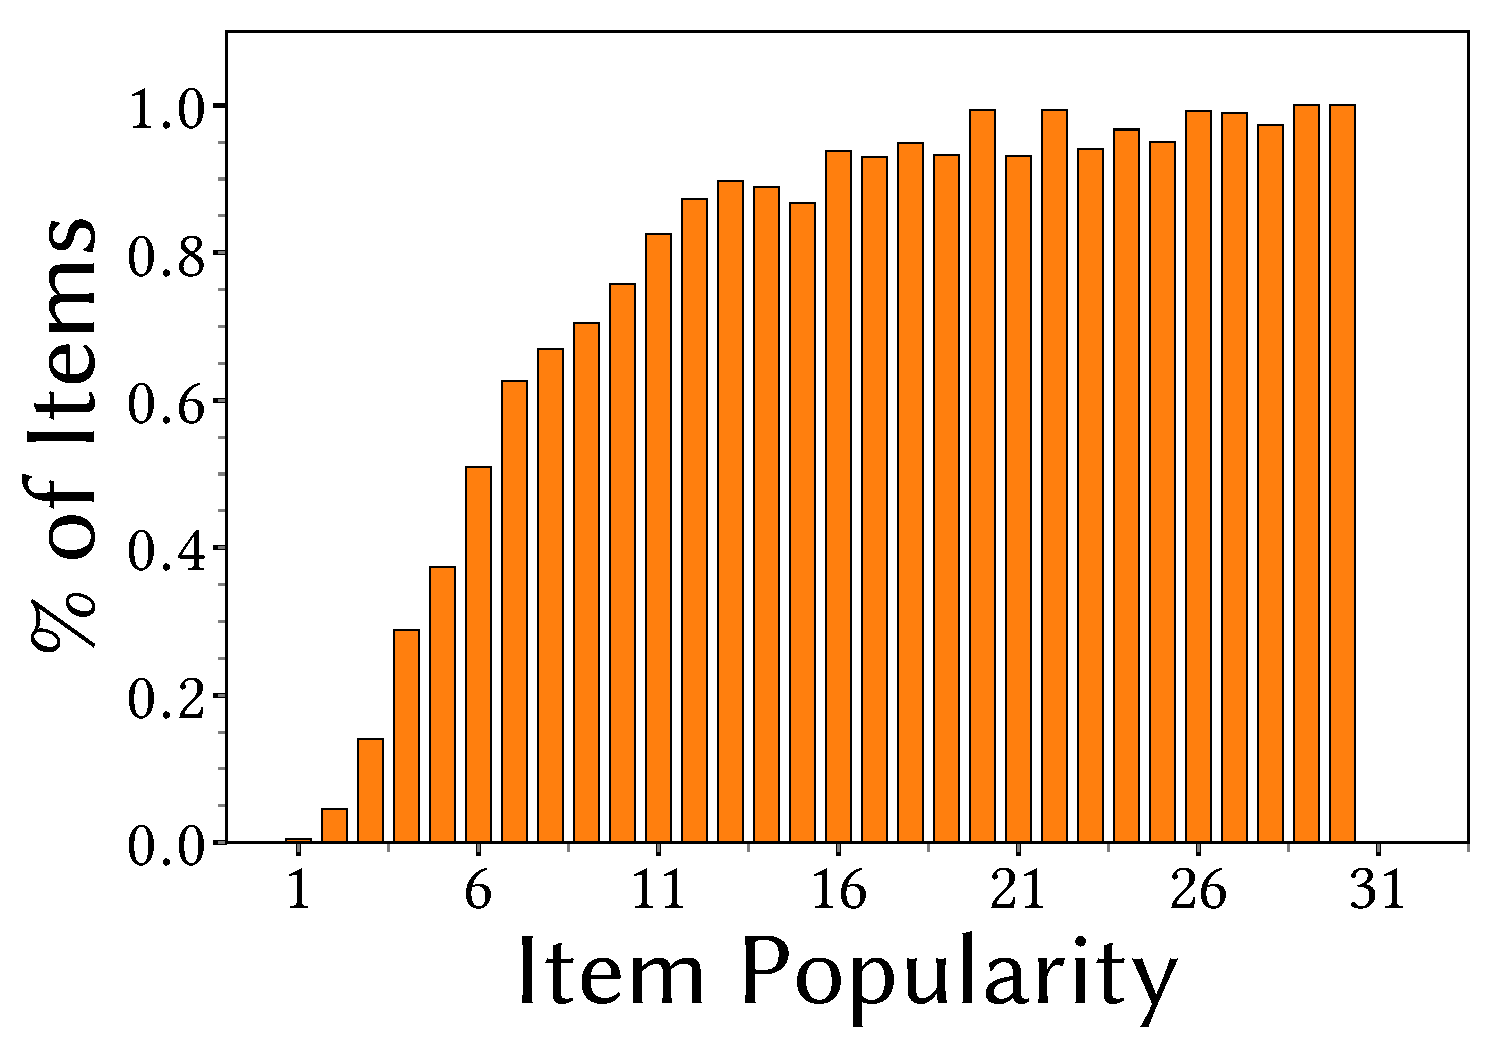
\includegraphics[height=4cm,width=0.3\linewidth]{figures/epinions_userSocial_Total_items_length.pdf}
  &
    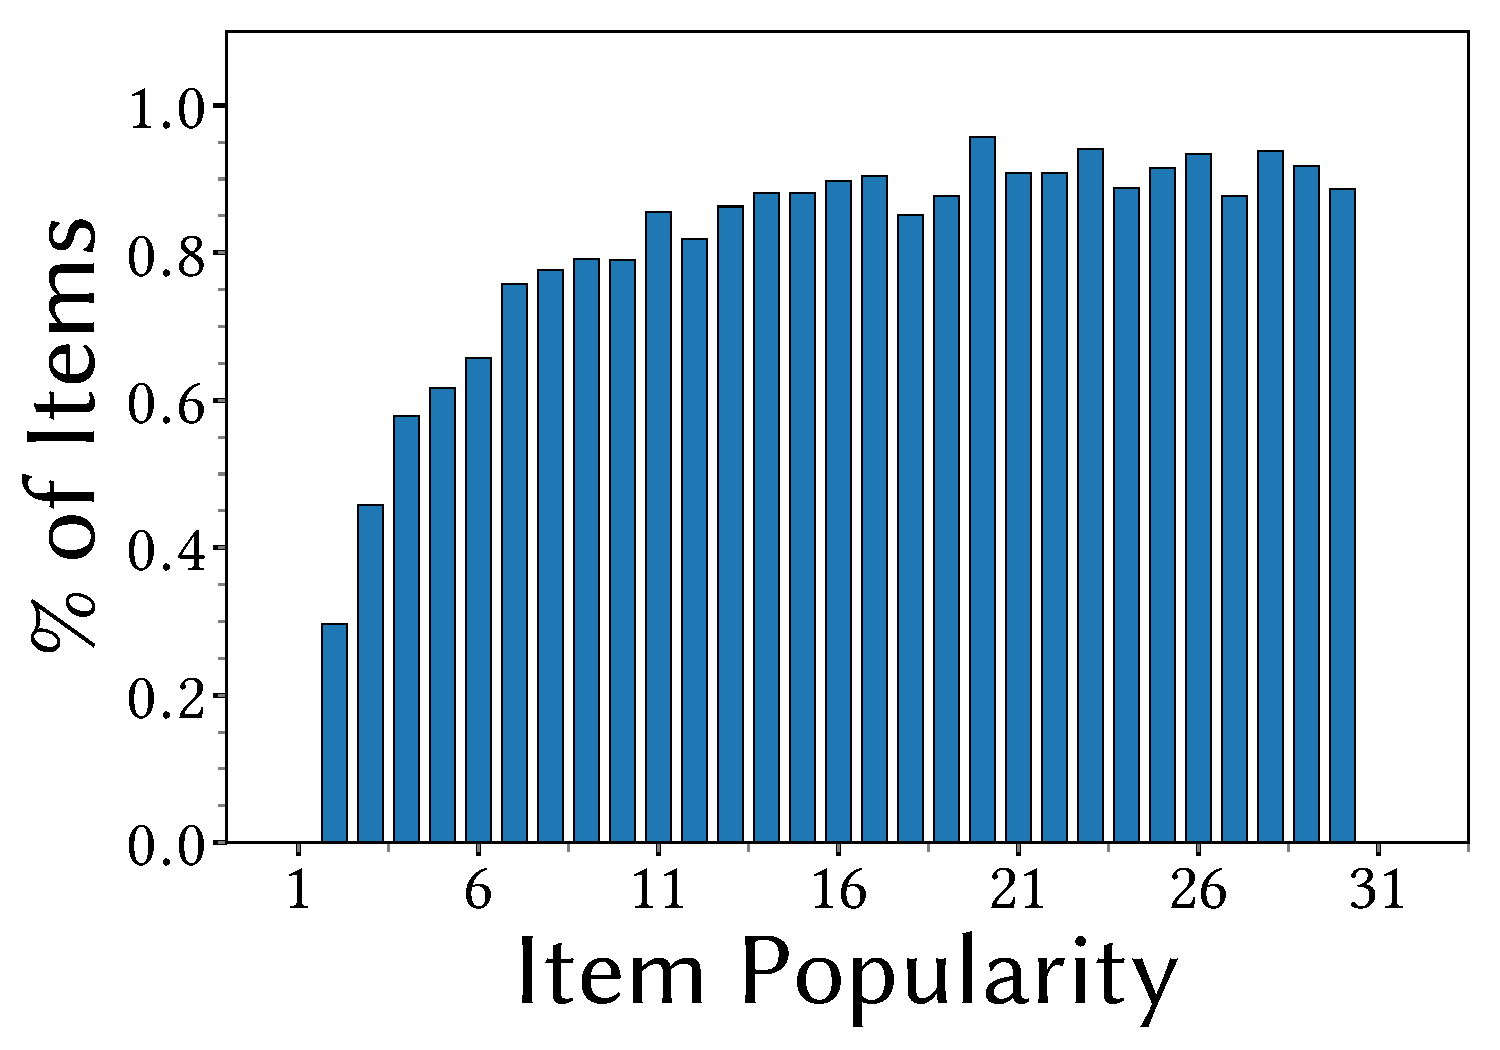
\includegraphics[height=4cm,width=0.3\linewidth]{figures/epinions_temporal_Total_items_length.pdf}\\
  \end{tabular}
  \caption{ Fraction of correct item predictions on test data by %GATRec model and its
  individual modules with different user sequence length, varying size of a user's social connections and varying item popularity. The item-similarity module performs better for rare items while the user-social module better models cold-start users.}
  \label{fig:analysis}
\end{figure}

Further, we evaluated individual modules with varying item popularity in the dataset, different sequence length for users, and varying size of a user's social graph for the Epinions dataset as shown in \Cref{fig:analysis}.
The user-social module is able to predict cold-start users better than the user-temporal module as it takes information from a user's social connections into account (top row). Note, the item-similarity module performs uniformly for different user sequence length as it does not contain any user information. Information about the past behavior of social connections (user-social module) improves performance compared to not using social connections (item-similarity module). Note that this effect increases with more friends and does not create noise as our attention model can distinguish between strong and weak connections (middle row).
The item-similarity module exploits item homophily in the user space and the feature space. Thus, it can accurately predict rarely reviewed items (in the left section of the figure, close to zero) better than the other two modules (bottom row).
Thus, our model provides an interpretable way of determining the importance of each of the factors used in our model through multiple experiments.


\subsection{Cold-Start Analysis} Combining different factors in each of the three modules helps to alleviate data sparsity and to predict for cold-start users effectively. To verify this claim, we evaluate our model in cold-start settings using a decreasing number of past available interactions for a user. \Cref{fig:ablationAUC}
provides our results with varying user sequence length compared to the baselines. Our model significantly outperforms the baselines modeling a subset of the factors for cold-start settings on all the three datasets reaffirming our claim.
Also, we observe that our model performs comparably for user history lengths 10 and above, while the performance drops for very short sequence length of 5. This further underlines that a user's temporal history is an essential cue for the recommendation.

\begin{figure}[tbh]
 \centering
 \begin{subfigure}[b]{\linewidth}
   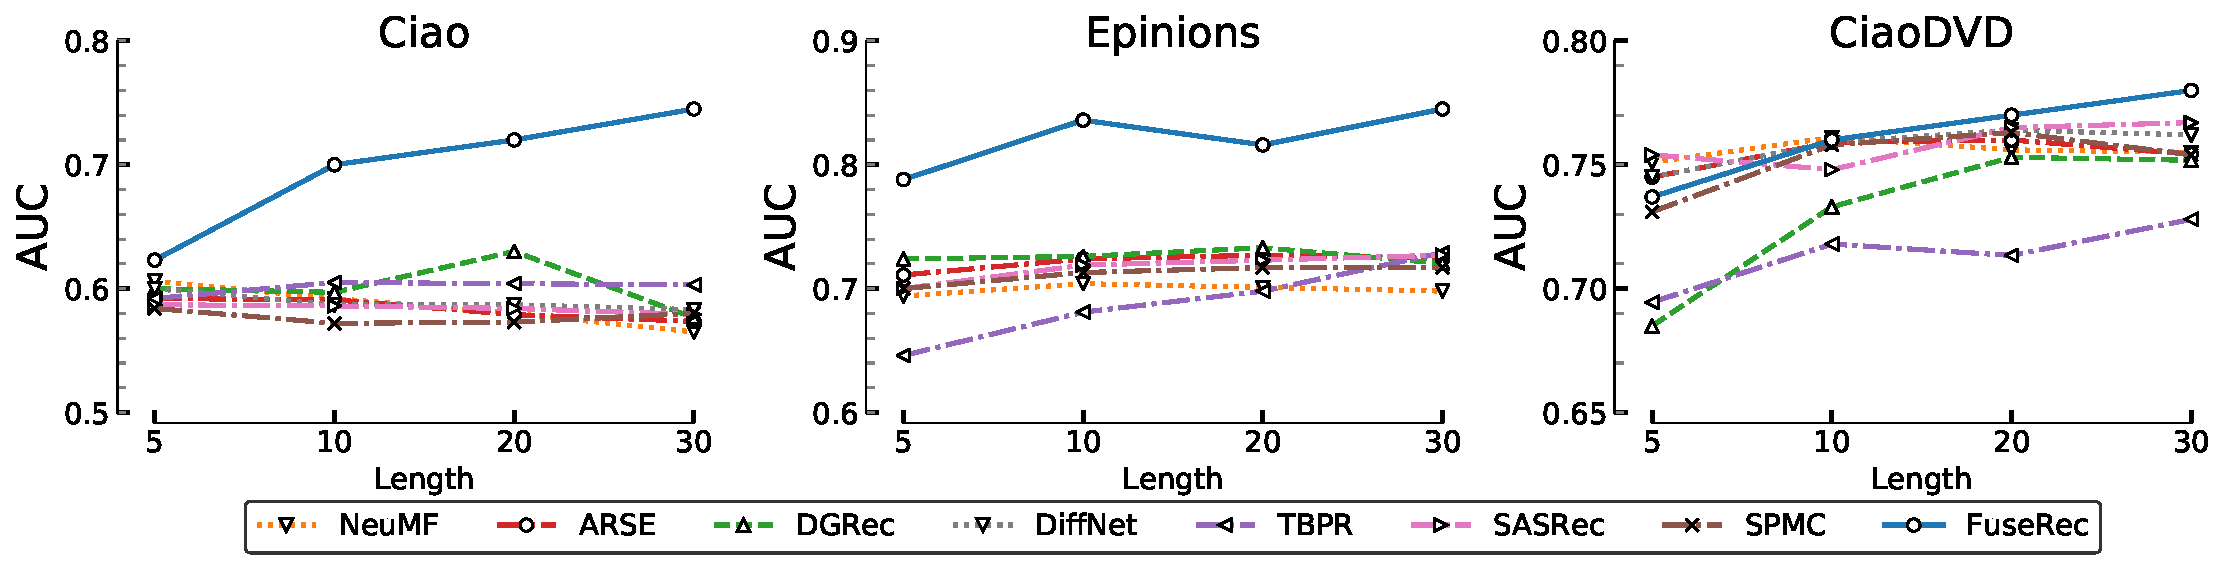
\includegraphics[width=1\linewidth]{figures/AUC.pdf}
 \end{subfigure}
 \caption{\label{fig:ablationAUC}AUC  over different number of  past interactions to mimic cold-start settings. Our model consistently outperforms all the social and temporal based baselines.}
\end{figure}

\subsection{Parameter Sensitivity}

\begin{table}[tbh]
    \centering
    \begin{tabular}{l c c c c c c } \toprule
     & \multicolumn{2}{c}{Ciao} & \multicolumn{2}{c}{Epinions} & \multicolumn{2}{c}{CiaoDVD}\\
     &  HR@10   &    AUC         &    HR@10   & AUC &    HR@10   & AUC \\ \hline
    No Attn & 0.313 & 0.707 & 0.536  & 0.697 & 0.515 & 0.742\\
    User\-side Attn & 0.356  & 0.719 &  0.531 & 0.729 & 0.532 & 0.747\\
    Item\-side Attn & 0.356 & 0.737 & 0.541 & 0.740 & 0.536 & 0.752\\
    \ours & 0.355 & 0.745 & 0.549 & 0.834 & 0.538 & 0.774\\
     \bottomrule
    \end{tabular}
\caption{Performance of our model without attention in the user-social and the item-similarity module. Attention in item-similarity module only performs better than only user-social module attention. }
\label{tab:attention}
\end{table}

\Cref{tab:attention} details performance results after removing attention from our user-social and item-similarity modules, respectively. The variant without attention on both the modules performs the worst. Comparing the user-social and item-similarity module: only using attention in the item-similarity module performs better than using attention in the user-social module exclusively. This is expected as the ties between similar items are weaker than explicit social connections between users. Thus, attention results in lower weights for noisy connections in the item-similarity module.

\begin{figure}[tbh]
 \centering
   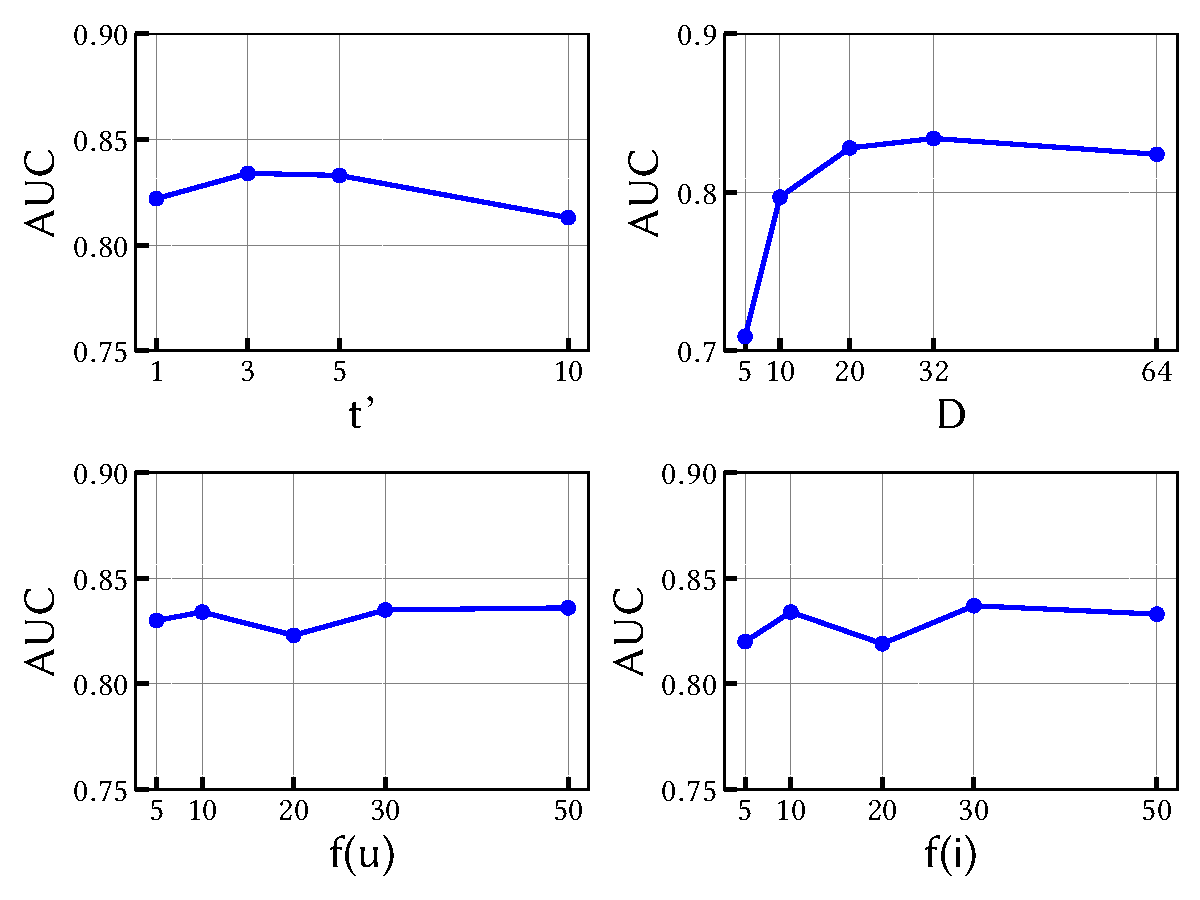
\includegraphics[scale=0.5]{figures/Ablation_new.pdf}
 \caption{Ablation results of different model hyper-parameters on Epinions datatset.}
 \label{fig:ablation}
\end{figure}

\Cref{fig:ablation} illustrates the performance of our model with different hyper-parameters on the Epinions dataset. For a user's friend's history length $t'$ (\Cref{eq:useragg}),  we observe: using fewer past interactions performs better. However, no change in performance is observed if $t'$ increases to more than the last five interacted items.
Increasing the size of the hidden dimension $D$ improves performance initially due to larger model capacity. However, results decline beyond a certain point due to overfitting.
For the user and item friend sample size, $F(u)$ (\Cref{eq:user}) and $F(i), F'(i)$  (\Cref{eq:item}) respectively, performance slightly increases with an increased size but plateaus for  sample sizes larger than 10.

\subsection{Induced relationships}

We further experimented with different graphs both in the User-Social and Item-Similarity module. In the user-social module, apart from the explicit social connections, we also induced another user graph based on similar preferences. Specifically, we computed k-nearest neighbors for each user using cosine similarity between their past item interactions. Similar to item graphs, we keep $k = 30$ for the user induced graph.
While for the item side, we experiment with two different graphs, one based on feature similarity between items, and another is based on frequent co-occurrence in the user's history.

Table \ref{tab:graph} details performance results when using different user and item graphs for all datasets. In general, using an induced user graph based on similar history performs competitively or slightly outperforms the explicit social graph. This reaffirms our hypothesis that connected users exhibit similar behavior. Note that computing similar users can be computationally expensive if the dataset is large.

\begin{table}[h]
    \centering
    \begin{tabular}{l l c c c c c c } \toprule
     & & \multicolumn{2}{c}{Ciao} & \multicolumn{2}{c}{Epinions} & \multicolumn{2}{c}{CiaoDVD}\\
     User Graph & Item Graph &  HR@10   &    AUC         &    HR@10   & AUC &    HR@10   & AUC \\ \hline
    Social & Co-Occurrence & 0.308 & 0.743 & 0.518  & 0.805 & 0.554 & 0.749\\
    Social & Feature & 0.292 & 0.709 & 0.520  & 0.827 & 0.537 & 0.747\\
    Induced & Both & 0.320 & 0.753 & --  & -- & 0.540 & 0.763\\
    Social & Both & 0.355 & 0.745 & 0.549 & 0.834 & 0.538 & 0.774\\
     \bottomrule
    \end{tabular}
\caption{Performance of our model with different graphs in the user-social and the item-similarity module. Induced relationships in the user graph fare little better than explicit social connections. In the item space also, item graph based on frequent co-occurrence in the user history is a better indicator of future item prediction. We could not extract induced user graph in Epinions because of out of memory error.}
\label{tab:graph}
\end{table}

In the item space, for Ciao and CiaoDVD, the co-occurrence graph performs better than the feature similarity graph. This competent performance is intuitive as most of the item collaborative filtering methods also leverage co-occurrence for providing recommendations. Besides, a similar item category may not be a strong signal of repeat user behavior as users tend to buy things across different categories.
